\documentclass[12pt]{article}\usepackage[]{graphicx}\usepackage[]{color}
%% maxwidth is the original width if it is less than linewidth
%% otherwise use linewidth (to make sure the graphics do not exceed the margin)
\makeatletter
\def\maxwidth{ %
  \ifdim\Gin@nat@width>\linewidth
    \linewidth
  \else
    \Gin@nat@width
  \fi
}
\makeatother

\definecolor{fgcolor}{rgb}{0.345, 0.345, 0.345}
\newcommand{\hlnum}[1]{\textcolor[rgb]{0.686,0.059,0.569}{#1}}%
\newcommand{\hlstr}[1]{\textcolor[rgb]{0.192,0.494,0.8}{#1}}%
\newcommand{\hlcom}[1]{\textcolor[rgb]{0.678,0.584,0.686}{\textit{#1}}}%
\newcommand{\hlopt}[1]{\textcolor[rgb]{0,0,0}{#1}}%
\newcommand{\hlstd}[1]{\textcolor[rgb]{0.345,0.345,0.345}{#1}}%
\newcommand{\hlkwa}[1]{\textcolor[rgb]{0.161,0.373,0.58}{\textbf{#1}}}%
\newcommand{\hlkwb}[1]{\textcolor[rgb]{0.69,0.353,0.396}{#1}}%
\newcommand{\hlkwc}[1]{\textcolor[rgb]{0.333,0.667,0.333}{#1}}%
\newcommand{\hlkwd}[1]{\textcolor[rgb]{0.737,0.353,0.396}{\textbf{#1}}}%
\let\hlipl\hlkwb

\usepackage{framed}
\makeatletter
\newenvironment{kframe}{%
 \def\at@end@of@kframe{}%
 \ifinner\ifhmode%
  \def\at@end@of@kframe{\end{minipage}}%
  \begin{minipage}{\columnwidth}%
 \fi\fi%
 \def\FrameCommand##1{\hskip\@totalleftmargin \hskip-\fboxsep
 \colorbox{shadecolor}{##1}\hskip-\fboxsep
     % There is no \\@totalrightmargin, so:
     \hskip-\linewidth \hskip-\@totalleftmargin \hskip\columnwidth}%
 \MakeFramed {\advance\hsize-\width
   \@totalleftmargin\z@ \linewidth\hsize
   \@setminipage}}%
 {\par\unskip\endMakeFramed%
 \at@end@of@kframe}
\makeatother

\definecolor{shadecolor}{rgb}{.97, .97, .97}
\definecolor{messagecolor}{rgb}{0, 0, 0}
\definecolor{warningcolor}{rgb}{1, 0, 1}
\definecolor{errorcolor}{rgb}{1, 0, 0}
\newenvironment{knitrout}{}{} % an empty environment to be redefined in TeX

\usepackage{alltt}
\usepackage[top=1.00in, bottom=1.0in, left=1.1in, right=1.1in]{geometry}
\renewcommand{\baselinestretch}{1.1}
\usepackage{graphicx}
\usepackage{natbib}
\usepackage{amsmath}
\bibliographystyle{..//refs/styles/besjournals.bst}
\renewcommand{\thetable}{S\arabic{table}}
\renewcommand{\thefigure}{S\arabic{figure}}
\usepackage{xr-hyper}
\externaldocument{shortest_reconciling}

\def\labelitemi{--}
\parindent=24pt
\title{Supplement: Reconciling historic hypotheses regarding flower-leaf sequences in temperate forests for fundamental and global change biology}
\IfFileExists{upquote.sty}{\usepackage{upquote}}{}
\begin{document}
\maketitle

\subsection*{Methods}
\subsubsection*{Climate Change and FLS:}
To evaluate how FLS patterns have changed over time in association with climate change we obtained phenological data for four European woody plant species with long term phenology records of both flower (BBCH 60) and leafout phenology (BBCH 11) from the Pan European Phenological Database \citep{PEP725}. We restricted the data set to include only stations with more than 50 years worth of data. For each species, we modeled the number of days between flowering and leafing as a function of time, using a hinge model with 1980 as break point in accordance with climate change models of \citet(). \textit{Lizzie do you have any citations for hinge models?} For each species, we display the pre-1980 mean and 95\% credible intervals of the time between flowering and leafing and the post-1980 change in mean time between phenophases that can be driven by climate change.

\subsubsection*{Defining FLS with MTSV and USFS data}
For these two, categorical, species level case studies, we converted verbal descriptions of flower-leaf sequences into a binary response variable. For our more inclusive "functional" definition of hysteranthy which allows for overlap between phenophases, we included species entries with descriptions \textit{"flowers before the leaves"}, \textit{"flowers before or with leaves"} and textit{"flowers with leaves"} as hysteranthous. Our more restrictive "physiological" hysteranthy definition only included species described as \textit{"flowers before the leaves"} as hysteranthous.\\

\noindent For modeling trait associates we chose three predictors to represent the three major FLS hypotheses; pollination syndrome, average flowering time and minimum precipitation levels across the species range. We obtained pollination syndrome and average flowering time information directly from the respective data sources and estimates of minimum precipitation across range from the USDA/NRCS Conservation Plants Characteristics database. We coded pollination syndrome as binary, biotic- or wind-pollinated and assigned known ambophilous species in the genus \textit{Salix} to the ancestral, biotic-pollinated, state of angiosperms. We re-coded flowering time as the average of the range of months of flowering reported in each data source.\\

\noindent For these case studies, we modeled associations between hysteranthy and the trait predictors with logistical regressions in phylogenetic generalized linear modeling framework \citep{Ives2010} using the R package ``phylolm" \citep{Ho2014}.Our models incorporated a published angiosperm phylogenetic tree \citep{Zanne2013} pruned to match the species list for each case study. Species found in the trait data set but not in the original phylogenetic tree were added to the pruned tree at the generic root. In total 32 species were added to the generic roots for the MTSV data set and eight for the USFS data set. We visualize phylogenetic patterning of FLS across the tree of each case study (Fig. \ref{fig:phylogeny}).

\noindent We ran the models with 599 bootstrapped re-sampling iterations for each data set \citep{Wilcox2010}. We standardized all predictors by subtracting the mean and dividing by two standard deviations to allow for a reasonable comparison of effect sizes between the binary and continuous predictors in this model \citep{Gelman2007}. 



\subsubsection*{Harvard Forest models}
For each individual tree per year in the data, we calculated the time between flowers opening and leaves reaching 75\% of their final size. To compare the inference from between catagorical and continuous measure of FLS we re-coded the HF continuous FLS measures as binary responses with positive values coded as hysteranthous and negative values as seranthous. These models used the same predictors as the MTSV and USFS datasets, except that we estimated the average flowering time directly from the HF data. All models the R package ``brms" \citep{Burkner2018} to estimate the relationship between FLS and the predictors with a phylogenetic mixed model in a Bayesian framework \citep{}. We ran each model with weak priors, a warmup of 3000 iterations and 4000 sampling iterations. As our primary goal was to directly compare the effects each predictor we standardized these variables to allow for a reasonable comparision between them {\citep{Gelman2007}. \\

\noindent To test examine the relationship between inter-annual variation in FLS and precipitation, we obtained precipitation records from the Shaler meteorological station at Harvard Forest \citep{}. We modeled the association between FLS variatation and annual precipiation with a complete pooling model. We also ran a model testing for interactions between the effects of annual precipitation and pollination syndrome on FLS.  As above, these models run with weak priors, a warmup of 3000 iterations and 4000 sampling iterations.\\

The three Harvard Forest models are detailed below:\\
\begin{enumerate}
\item \underline{Categorical model}:\\
Pr(y_i &=1) &= logit^{-1} (\alpha_{sp[i]} + \beta_{pollination syndrome}X_1_[_1_] + \beta_{flowering time}X_2_[_i_] + \beta_{min. precipitation}X_3_[_i_] +\beta_{pollination syndrome}:\beta_{flowering time}X_4_[_i_]+\beta_{pollination syndrome}:\beta_{min. precipitation}X_5_[_i_]+ \beta_{flowering time}:\beta_{min. precipitation}X_6_[_i_] + \epsilon_i)\\

\noindent $\alpha$ was modeled at the species level, as follows:\\
\alpha_{sp} & \sim N(\mu_{\alpha}, \sigma_{\alpha}) \\

\item \underline{Continuous model}: \\
y_i &= \alpha_{sp[i]} + \beta_{pollination syndrome}X_1_[_i_] + \beta_{flowering time}X_2_[_i_] + \beta_{min. precipitation}X_3_[_i_] +\beta_{pollination syndrome}:\beta_{flowering time}X_4_[_i_]+\beta_{pollination syndrome}:\beta_{min. precipitation}X_5_[_i_]+ \beta_{flowering time}:\beta_{min. precipitation}X_6_[_i_] + \epsilon_i\\
\epsilon_i & \sim N(0,\sigma^2_y) \\ %I Think this is wrong and should reflect the phyogeny

\noindent with:\\
\alpha_{sp} & \sim N(\mu_{\alpha}, \sigma_{\alpha}) \\

\item \underline{Inter-annual model}:\\
y_i &= \alpha_{i} + \beta_{annual precipitation}X_1[i] + \epsilon_i\\
\epsilon_i & \sim N(0,\sigma^2_y) \\

\end{enumerate}
\indent We calculated the marginal effects for the Harvard Forest continuous model using the R-package ``ggeffects" \citep{Ludecke2018}.\\

\noindent Though we make broad comparisons between the HF and MTSV/USFS case studies, differences in data structure between the datasets required us to use alternative modeling frameworks. The MTSV and USFS data provide one response variable for each species while the HF data contains intra-specific differences in FLS, providing several different response values per species. The current phylogenetic generalized linear model framework can only fit models with one response value per species, while the phylogenetic mixed model in brms over-fits models with this kind of data structure (Paul Burkner, personal communication) and performs better on multi-response per species datasets like HF. We ran both model types on each case study and while they do yield different absolute estimates, the patterns we found were consistent across each framework, and we report results from the most acurate model for each dataset.\\

\subsubsection{Phylogenetic signals}
For all categorical specifications of FLS (MTSV, USFS and HF), we assessed the phylgenetic structure of hysteranthous flowering in all  with Fritz's D-statistic \citep{FRITZ2010} using the ``Caper package" \citep{Orme2013} in R. Fritz's D calculates the sum of changes in estimated node values of a binary trait along edges in a phylogeny and compares this observed value to both a model of Phylogenetic randomness and Brownian threshold model. The means of the two data simulations scale values of D to set points of 0 (as phylogenetically conserved) and 1 (random)  \citep{Orme2013}.\\

\noindent For the qunatitative Harvard Forest model, we estimated a phylogenetic signal (lambda)

\section*{Supplimental Tables and Figures}

\begin{figure}[h!]
    \centering
 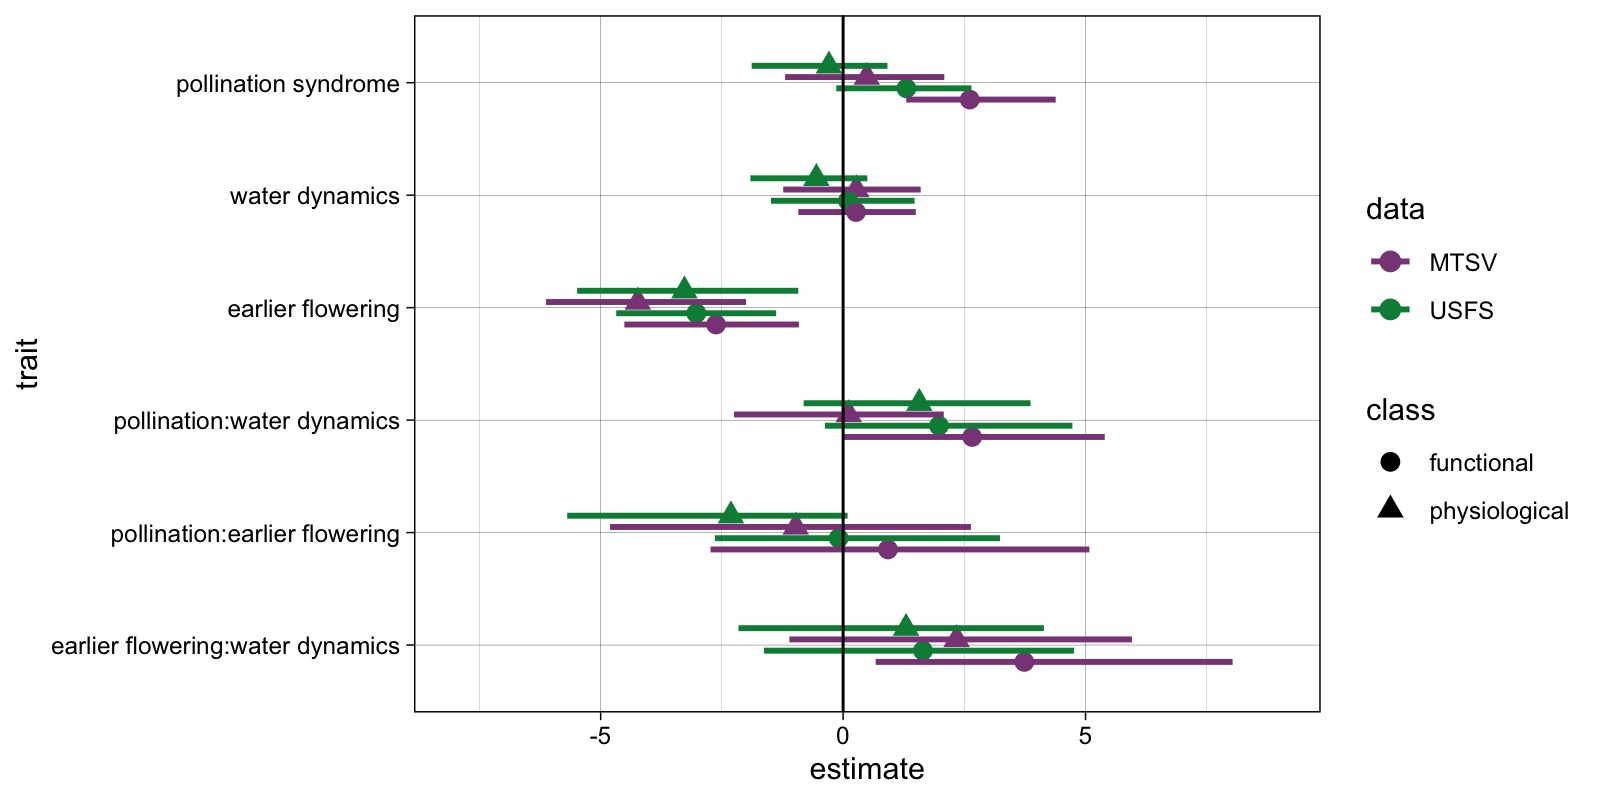
\includegraphics[width=\textwidth]{..//MTSV_USFS.jpeg} 
    \caption{\textbf{Mean estimates of the effects of FLS predictors on the likehilood a species is hysteranthous vary across datasets and definitions of FLS.}  We used phylogenetic adjustments and standardized units to make a basic comparison of two datasets and classes (physiological= no overlap between flowering and leafing, functional= moderate overlap) of FLS. While there is some agreement accross models (strong effects of flowering time, no consistant effect interactions between predictors), the effect of other predictors (pollination syndrome, water dynamics) were highly sensitive to how data were defined, biasing any inference from models and compromising the ability to validate the exisitng FLS hypotheses. Lines represent 95\% bootstrap intervals.}
    \label{fig:muplots.USMT}
\end{figure}

\begin{figure}[h!]
    \centering
 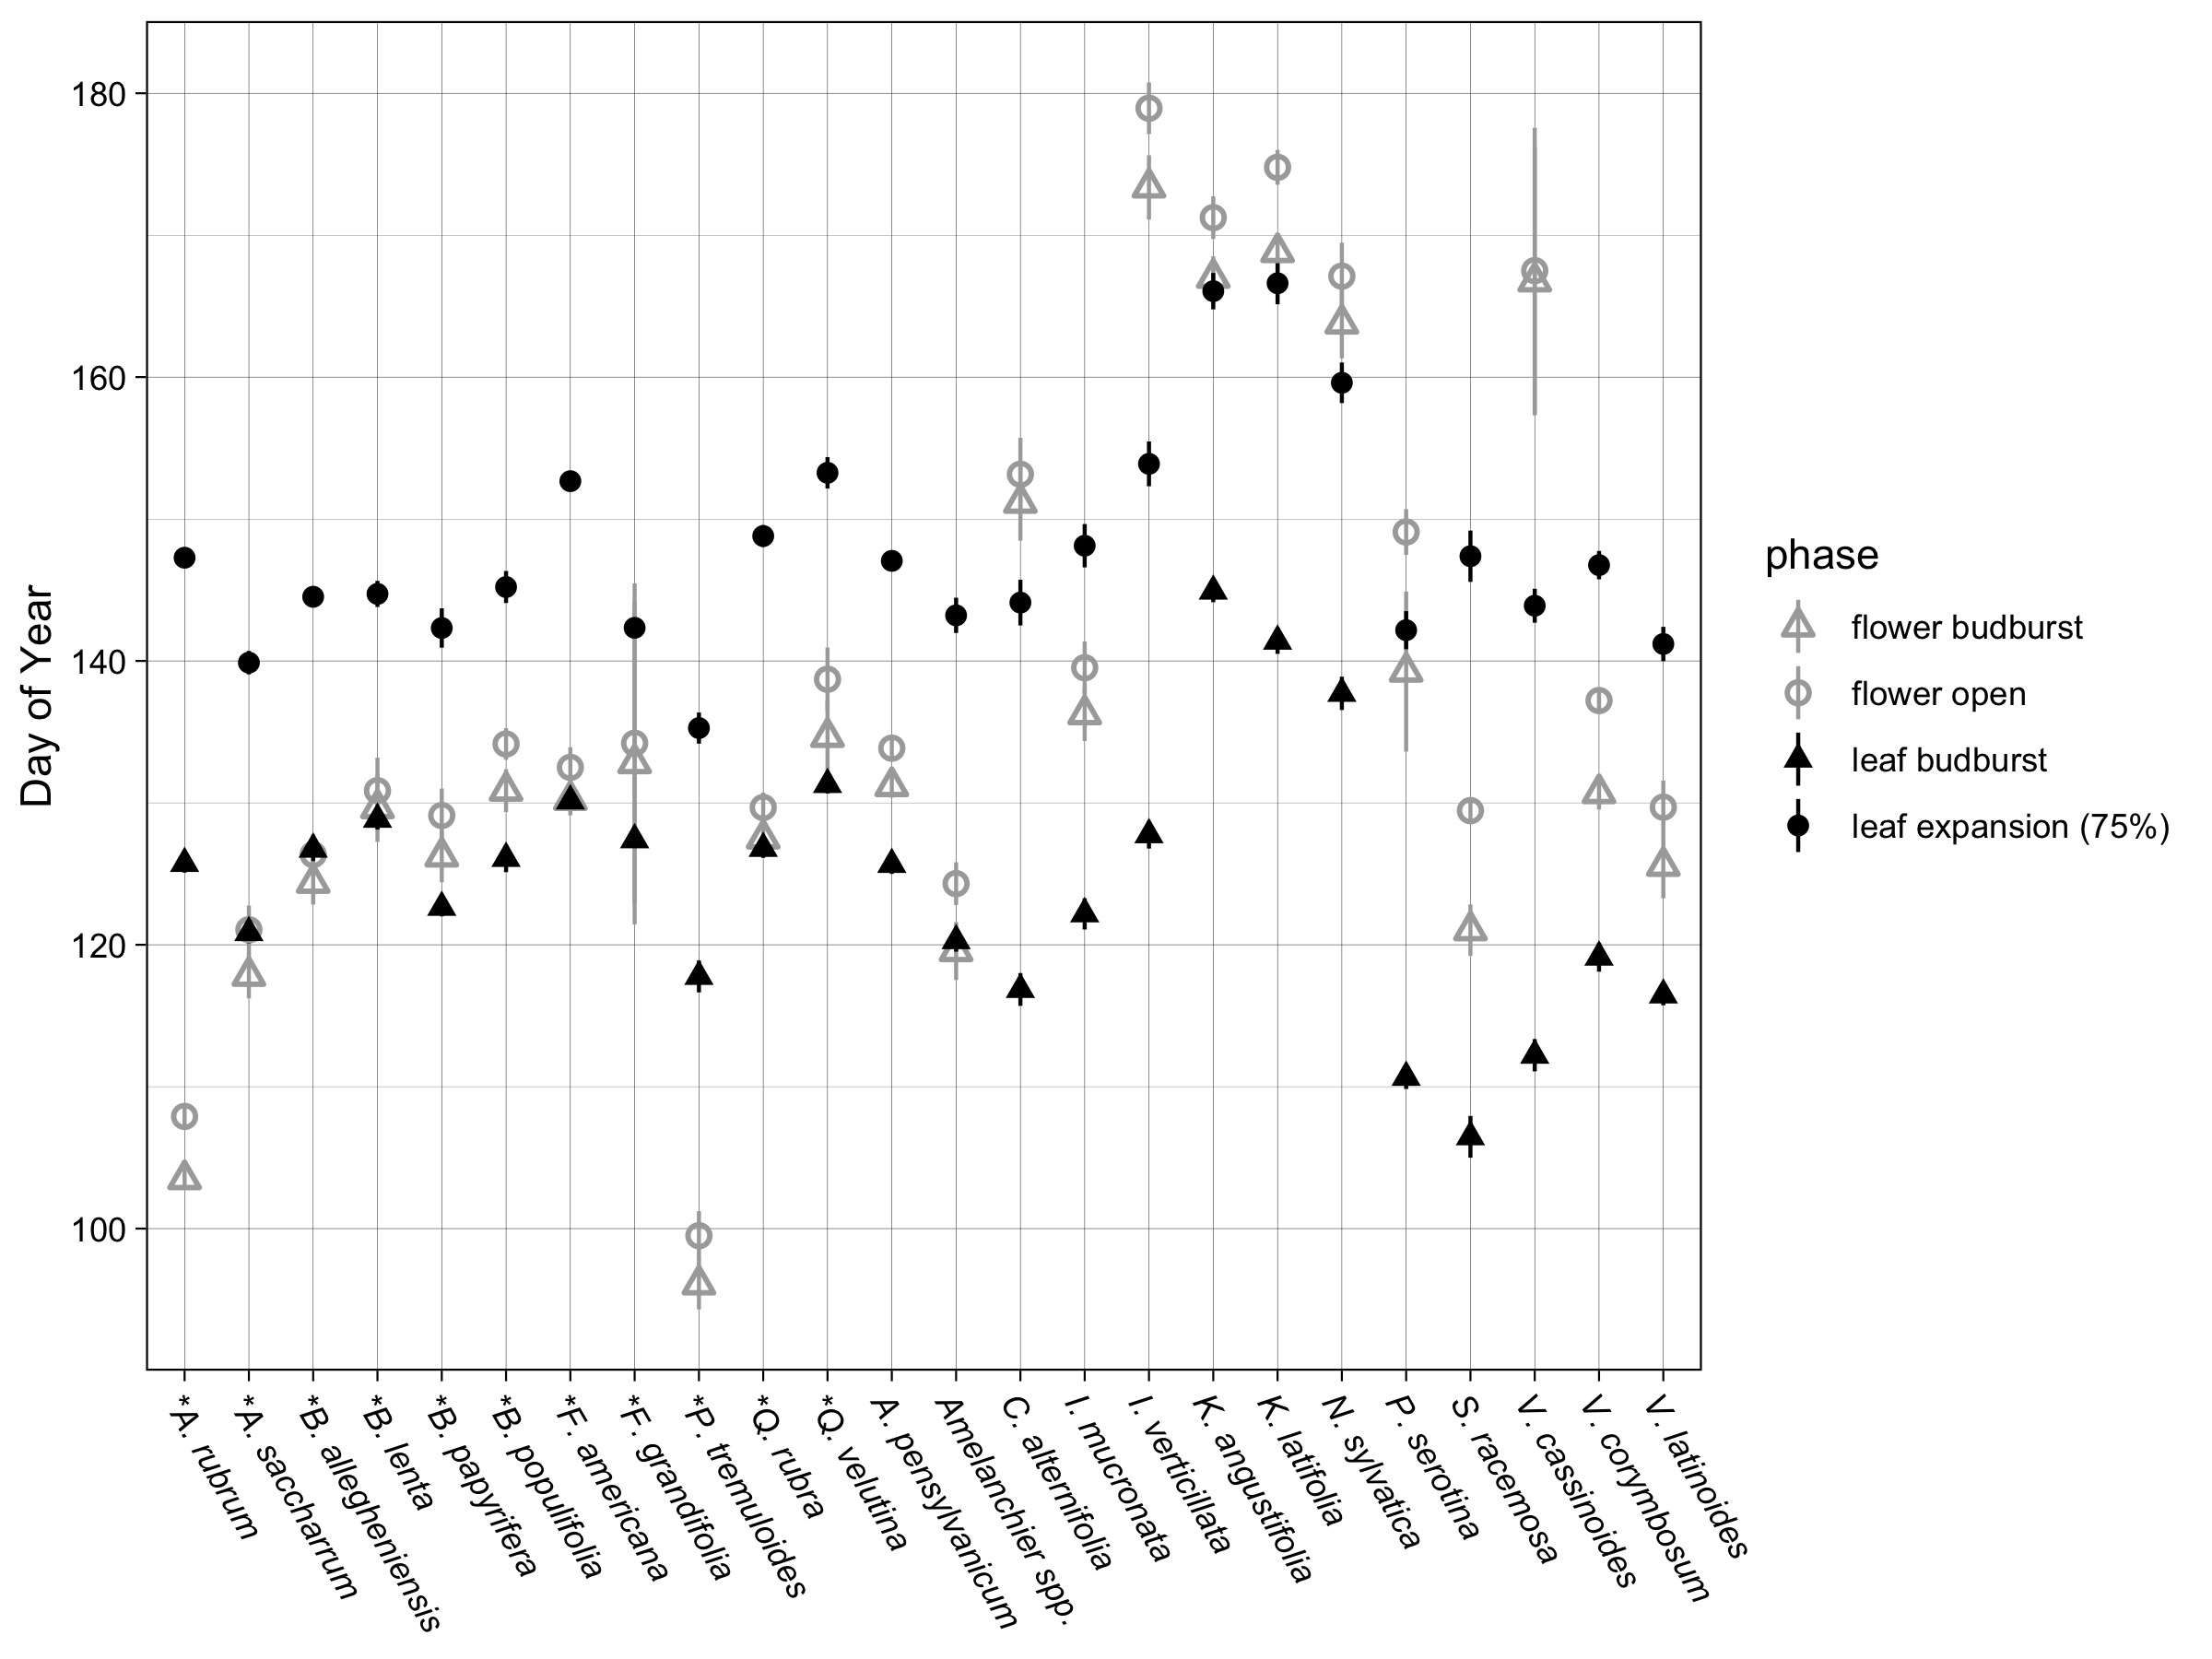
\includegraphics[width=\textwidth]{..//HarvardForest/HFmeans_expanded.jpeg} 
    \caption{\textbf{Quantitative FLS patterns for woody plants at Harvard Forest in Pertersham, MA.} Because phenological sequences consist of serveral sub-stages if is difficult to unambiguously catagorize many species into the currently FLS categories. }
    \label{fig:HFmeans}
\end{figure}

\pagebreak
\begin{figure}

  \caption{\textbf{The phylogenetic signal for FLS varies between datasets and is sensitive to how FLS patterns are categorized. The black vertical line show the the Fritz's D statistic estimated from the data,}}
    \label{fig:Dstat}
    \end{figure}

\pagebreak
\begin{figure}[H]

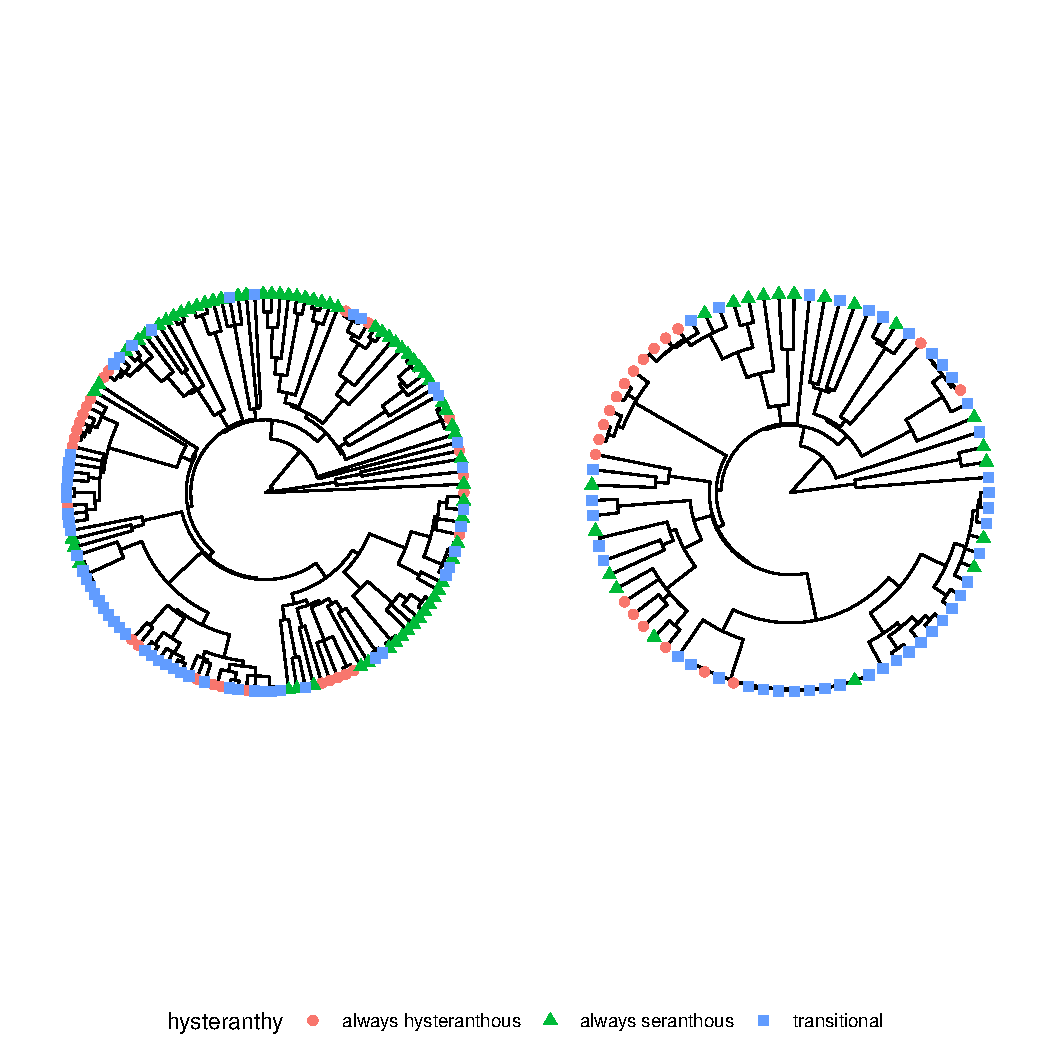
\includegraphics[width=7.5in]{figure/Code_chunk_Minimal_example3-1} 

   
  \caption{\textbf{Phylogenetic structure of FLS in MTSV and USFS varies significantly depending on how FLSs are defined.} Many species get re-assigned to either hysteranthy or seranthy depending on whether FLS is defined functionally (partial overlap between flowering and leafing allowed) or physiologically (no overlap between flowering and leafing allowed) (blue squares). This modeling choice dramatically alters FLS patterning across the tree, resulting in an unstable phylogentical signal for this trait.}
    \label{fig:phylogeny}
    \end{figure}
  
  
\pagebreak
\bibliography{..//refs/hyst_outline.bib}
\end{document}
